\documentclass[%keepfline,
booktitle=工科のための数学,
a5/13Q,
uplatex,
dvipdfmx,
jis2004,%%or jis2000
useotf,
]{kbdbook}
\usepackage[OT1,T1]{fontenc}
\usepackage{textcomp}
\usepackage{lmodern}
\usepackage[deluxe]{otf}
% 設定確認用
%\usepackage{KBtexrpara}%% 組版パラメータ
%\usepackage{baselinehead}%% baselineの表示

%% 和文の割り当て
\usepackage[ipaex,
%   baseMincho = A-OTF-RyuminPr6-Regular.otf,
%   baseGothic = A-OTF-GothicBBBPr6-Medium.otf,
%   mcl =,
%   mcb =,
%   gtb =,
%   eb = ,
%   mg* = ,
%   mgscale=.5
]{KBDaddjfont}
\usepackage{amsmath}
\usepackage{makeidx}
\usepackage{bm}
\usepackage{graphicx,xcolor}
\usepackage{nccmath}%% 数式で\begin{fleqn}[0pt]など
\usepackage{enumitem}%% 箇条書きのカスタマイズ
\usepackage{emathMw}% 回り込み
\usepackage{macros}
\makeindex

\graphicspath{{./fig/}}

%% 章ごとにファイル分割(必要に応じて加減)
\includeonly{
	Chap01,
	Chap02,
	Chap03,
	Chap05,
	Chap06,
	}

\begin{document}
\frontmatter
   \tableofcontents
\mainmatter
%% 見本ファイル.不要になったら削除してください.
\chapter{統計的推定}

%% 
\begin{abstract}
\S4 の変数変換式の証明は完全ではない.完全な証明はあとがきの文献を見ていただきたい.多変数関数の積分のことを\textbf{重積分}ともいう.
\end{abstract}


\section{分布の特性を数値的尺度で表す度で表す}
の変数変換式の証明は
\subsection{数列の極限}


23歳のとき,パスカルの実証精神はトリチュリの真空実験を発展させ,大気圧は高さによって決まることを示しました.『真空に関する新実験』(1647)において,パスカルはス
\subsubsection{2項分布の正規近似}

%% QEDあり
\begin{証明}
23歳のとき,パスカルの実証精神はトリチュリの真空実験を発展させ,大気圧は高さによって決まることを示しました.『真空に関する新実験』(1647)において,パスカルはスコニュの旧家で,祖父マルタンは富裕な商家の出であり,騎士の称号を授与されました.\end{証明}

\begin{figure}[h!]
\centering
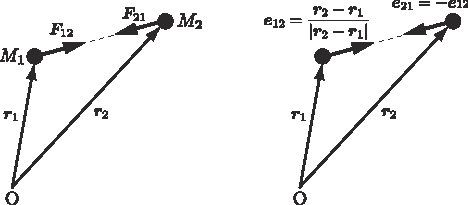
\includegraphics{2-3_1.pdf}
\caption{}\label{fig:C1:01}
\end{figure}
%% QEDなし
\begin{証明*}
23歳のとき,パスカルの実証精神はトリチュリの真空実験を発展させ,大気圧は高さによって決まることを示しました.『真空に関する新実験』(1647)において,パスカルはスコニュの旧家で,祖父マルタンは富裕な商家の出であり,騎士の称号を授与されました.\begin{align*}
\bm{r}&=x\,\bm{e}_x+y\,\bm{e}_y+z\,\bm{e}_z\ ,\\
\bm{v}&=v_x\,\bm{e}_x+v_y\,\bm{e}_y+v_z\,\bm{e}_z\ ,\tag*{\QED}
\end{align*}
\end{証明*}

\begin{定義}
23歳のとき,パスカルの実証精神はトリチュリの真空実験を発展させ,大気圧は高さによって決まることを示しました.『真空に関する新実験』(1647)において,パスカルはスコニュの旧家で,祖父マルタンは富裕な商家の出であり,騎士の称号を授与されました.\end{定義}

\begin{定義}
23歳のとき,パスカルの実証精神はトリチュリの真空実験を発展させ,大気圧は高さによって決まることを示しました.『真空に関する新実験』(1647)において,パスカルはスコニュの旧家で,祖父マルタンは富裕な商家の出であり,騎士の称号を授与されました.\end{定義}

\begin{定理}
23歳のとき,パスカルの実証精神はトリチュリの真空実験を発展させ,大気圧は高さによって決まることを示しました.『真空に関する新実験』(1647)において,パスカルはスコニュの旧家で,祖父マルタンは富裕な商家の出であり,騎士の称号を授与されました.\end{定理}
\begin{定理}
23歳のとき,パスカルの実証精神はトリチュリの真空実験を発展させ,大気圧は高さによって決まることを示しました.『真空に関する新実験』(1647)において,パスカルはスコニュの旧家で,祖父マルタンは富裕な商家の出であり,騎士の称号を授与されました.\end{定理}
\begin{figure}[t!]
\centering
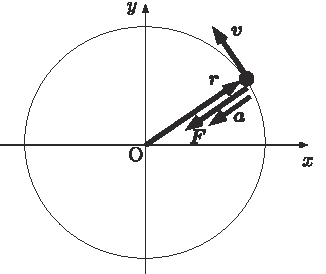
\includegraphics{5-1_2.pdf}
\caption{}\label{fig:C1:02}
\end{figure}

\begin{補題}
23歳のとき,パスカルの実証精神はトリチュリの真空実験を発展させ,大気圧は高さによって決まることを示しました.『真空に関する新実験』(1647)において,パスカルはスコニュの旧家で,祖父マルタンは富裕な商家の出であり,騎士の称号を授与されました.\end{補題}
\begin{補題}
23歳のとき,パスカルの実証精神はトリチュリの真空実験を発展させ,大気圧は高さによって決まることを示しました.『真空に関する新実験』(1647)において,パスカルはスコニュの旧家で,祖父マルタンは富裕な商家の出であり,騎士の称号を授与されました.\end{補題}


\begin{系}
23歳のとき,パスカルの実証精神はトリチュリの真空実験を発展させ,大気圧は高さによって決まることを示しました.『真空に関する新実験』(1647)において,パスカルはスコニュの旧家で,祖父マルタンは富裕な商家の出であり,騎士の称号を授与されました.\end{系}
\begin{系}
23歳のとき,パスカルの実証精神はトリチュリの真空実験を発展させ,大気圧は高さによって決まることを示しました.『真空に関する新実験』(1647)において,パスカルはスコニュの旧家で,祖父マルタンは富裕な商家の出であり,騎士の称号を授与されました.\end{系}

\begin{命題}
23歳のとき,パスカルの実証精神はトリチュリの真空実験を発展させ,大気圧は高さによって決まることを示しました.『真空に関する新実験』(1647)において,パスカルはスコニュの旧家で,祖父マルタンは富裕な商家の出であり,騎士の称号を授与されました.\end{命題}
\begin{命題}
23歳のとき,パスカルの実証精神はトリチュリの真空実験を発展させ,大気圧は高さによって決まることを示しました.『真空に関する新実験』(1647)において,パスカルはスコニュの旧家で,祖父マルタンは富裕な商家の出であり,騎士の称号を授与されました.\end{命題}

\begin{注意}
23歳のとき,パスカルの実証精神はトリチュリの真空実験を発展させ,大気圧は高さによって決まることを示しました.『真空に関する新実験』(1647)において,パスカルはスコニュの旧家で,祖父マルタンは富裕な商家の出であり,騎士の称号を授与されました.\end{注意}
\begin{注意}
23歳のとき,パスカルの実証精神はトリチュリの真空実験を発展させ,大気圧は高さによって決まることを示しました.『真空に関する新実験』(1647)において,パスカルはスコニュの旧家で,祖父マルタンは富裕な商家の出であり,騎士の称号を授与されました.\end{注意}
\begin{例}[ポアッソン分布のパラメータ]
ある:任意に与えられた正の数$\varepsilon$に対してある正の数$\sigma$をとると,
$A$の2点$\bm{x},\bm{y}$が$d(\bm{x},\bm{y})<\sigma$をみたせば,$|f(\bm{f})-f(\bm{y})|<\varepsilon$が成り立つ,
\end{例}
\begin{例}[ポアッソン分布のパラメータ]
ある:任意に与えられた正の数$\varepsilon$に対してある正の数$\sigma$をとると,
$A$の2点$\bm{x},\bm{y}$が$d(\bm{x},\bm{y})<\sigma$をみたせば,$|f(\bm{f})-f(\bm{y})|<\varepsilon$が成り立つ,
\end{例}
23歳のとき,パスカルの実証精神はトリチュリの真空実験を発展させ,大気圧は高さによって決まることを示しました.『真空に関する新実験』(1647)において,パスカルはスコニュの旧家で,祖父マルタンは富裕な商家の出であり,騎士の称号を授与されました.
\begin{コラム}
\noindent
\textbf{ド・メレとの邂逅}\par
23歳のとき,パスカルの実証精神はトリチュリの真空実験を発展させ,大気圧は高さによって決まることを示しました.『真空に関する新実験』(1647)において,パスカルはスコニュの旧家で,祖父マルタンは富裕な商家の出であり,騎士の称号を授与されました.
23歳のとき,パスカルの実証精神はトリチュリの真空実験を発展させ,大気圧は高さによって決まることを示しました.『真空に関する新実験』(1647)において,パスカルはスコニュの旧家で,祖父マルタンは富裕な商家の出であり,騎士の称号を授与されました.
23歳のとき,パスカルの実証精神はトリチュリの真空実験を発展させ,大気圧は高さによって決まることを示しました.『真空に関する新実験』(1647)において,パスカルはスコニュの旧家で,祖父マルタンは富裕な商家の出であり,騎士の称号を授与されました.
23歳のとき,パスカルの実証精神はトリチュリの真空実験を発展させ,大気圧は高さによって決まることを示しました.『真空に関する新実験』(1647)において,パスカルはスコニュの旧家で,祖父マルタンは富裕な商家の出であり,騎士の称号を授与されました.23歳のとき,パスカルの実証精神はトリチュリの真空実験を発展させ,大気圧は高さによって決まることを示しました.『真空に関する新実験』(1647)において,パスカルはスコニュの旧家で,祖父マルタンは富裕な商家の出であり,騎士の称号を授与されました.23歳のとき,パスカルの実証精神はトリチュリの真空実験を発展させ,大気圧は高さによって決まることを示しました.『真空に関する新実験』(1647)において,パスカルはスコニュの旧家で,祖父マルタンは富裕な商家の出であり,騎士の称号を授与されました.23歳のとき,パスカルの実証精神はトリチュリの真空実験を発展させ,大気圧は高さによって決まることを示しました.『真空に関する新実験』(1647)において,パスカルはスコニュの旧家で,祖父マルタンは富裕な商家の出であり,騎士の称号を授与されました.
\end{コラム}

\begin{章末問題}
\item[問題1] 23歳のとき,パスカルの実証精神はトリチュリの真空実験を発展させ,大気圧は高さによって決まることを示しました.『真空に関する新実験』(1647)において,パスカルはスコニュの旧家で,祖父マルタンは富裕な商家の出であり,騎士の称号を授与されました.
\begin{enumerate}
\item 23歳のとき,パスカルの実証精神はトリチュリの真空実験を発展させ,大気圧は高さによって決まることを示しました.『真空に関する新実験』(1647)において,パスカルはスコニュの旧家で,祖父マルタンは富裕な商家の出であり,騎士の称号を授与されました.
\item コニュの旧家で,
\item コニュの旧家で,
\end{enumerate}
\item[問題2] コニュの旧家で,
\item[問題3] コニュの旧家で,
\end{章末問題}

\index{こてんぶつりがく@古典物理学}
\index{ちいさいものとおおきいもの@小さいものと大きいもの}
\index{Planckのりょうしかせつ@Planckの量子仮説}
\index{ねつふくしゃ@熱輻射}
\index{Planckていすう@Planck定数}
\index{そでんか@素電荷}
\index{でんししつりょう@電子質量}
\index{しんくうのゆうでんりつ@真空の誘電率}
\index{Einsteinのこうりょうしかせつ@Einsteinの光量子仮説}
\index{こうし@光子}
\index{こうりょうしかせつ@光量子仮説}
\index{Einsteinのかんけいしき@Einsteinの関係式}
\index{こうでんこうか@光電効果}
\index{げんしのあんていせい@原子の安定性}
\index{げんしすぺくとる@原子スペクトル}
\index{げんしかく@原子核}
\index{Rydbergのこうしき@Rydbergの公式}
\index{せんすぺくとる@線スペクトル}
\index{おびすぺくとる@帯スペクトル}
\index{Rydbergすう@Rydberg数}
\index{Lymanけいれつ@Lyman系列}
\index{Balmerけいれつ@Balmer系列}
\index{Paschenけいれつ@Paschen系列}
\index{Bohrのりろん@Bohrの理論}
\index{ていじょうじょうたい@定常状態}
\index{たいおうげんり@対応原理}
\index{ていじょうじょうたい@定常状態}
\index{せんい@遷移}
\index{Bohrのしんどうすうじょうけん@Bohrの振動数条件}
\index{たいおうげんり@対応原理}
\index{かくうんどうりょう@角運動量}
\index{へんすうぶんりかのうなけい@変数分離可能な系}
\index{Bohr-Sommerfeldのりょうしかじょうけん@Bohr--Sommerfeldの量子化条件}
\index{ぎょうれつりきがく@行列力学}
\index{ぎょうれつりきがく@行列力学}
\index{はどうりきがく@波動力学}
\index{de Broglieはちょう@de Broglie波長}
\index{ぶっしつは@物質波}
\index{de Broglieのかんけい@de Broglieの関係}
\index{かくりつかいしゃく@確率解釈}
\index{Bohr-Sommerfeldのりょうしかじょうけん@Bohr--Sommerfeldの量子化条件}
\index{へんぶんげんり@変分原理}
\index{Hamilton-Jacobiほうていしき@Hamilton--Jacobi方程式}
\index{きかこうがく@幾何光学}
\index{Fermatのげんり@Fermatの原理}
\index{はどうのきかこうがくきんじ@波動の幾何光学近似}
\index{Fermatのげんり@Fermatの原理}
\index{そうきょくがたのはどうほうていしき@双曲型の波動方程式}
\index{たんしょくは@単色波}
\index{あいこなあるほうていしき@アイコナール方程式}
\index{こうせん@光線}
\index{Fermatのげんり@Fermatの原理}
\index{さいしょうさようのげんり@最小作用の原理}
\index{Maupertuisのげんり@Maupertuisの原理}
\index{Hamilton-Jacobiほうていしき@Hamilton--Jacobi方程式}
\index{さいしょうさようのげんり@最小作用の原理}
\index{Maupertuisのげんり@Maupertuisの原理}
\index{Jacobiのげんり@Jacobiの原理}
\index{Fermatのげんり@Fermatの原理}
\index{じかんにいぞんするSchrodingerほうていしき@時間に依存するSchr\"{o}dinger方程式}
\index{Hamiltonのとくせいかんすう@Hamiltonの特性関数}
\index{Hamilton-Jacobiほうていしき@Hamilton--Jacobi方程式}
\index{de Broglieは@de Broglie波}
\index{かくりつしんぷく@確率振幅}
\index{de Broglieは@de Broglie波}
\index{Schrodingerほうていしき@Schr\"{o}dinger方程式}
\index{Hamilton-Jacobiほうていしき@Hamilton--Jacobi方程式}
\index{きかこうがくきんじ@幾何光学近似}
\index{じかんにいぞんするSchrodingerほうていしき@時間に依存するSchr\"{o}dinger方程式}
\index{Einstein-de Broglieのじょうけん@Einstein--de Broglieの条件}
\index{じかんにいぞんするSchrodingerほうていしき@時間に依存するSchr\"{o}dinger方程式}
\index{Einstein-de Broglieのじょうけん@Einstein--de Broglieの条件}
\index{Einstein-de Broglieのじょうけん@Einstein--de Broglieの条件}
\index{Laplacian}
\index{じかんにいぞんするSchrodingerほうていしき@時間に依存するSchr\"{o}dinger方程式}
\index{かくりつかいしゃく@確率解釈}
\index{みくろなけい@ミクロな系}
\index{そうたいひんど@相対頻度}
\index{かくりつ@確率}
\index{かくりつみつど@確率密度}
\index{きかくか@規格化}
\index{とのむらあきら@外村彰}
\index{2じょうかせきぶん@2乗可積分}
\index{かくりつしんぷく@確率振幅}
\index{せきじしょうのかくりつ@積事象の確率}
\index{はいいくうかん@配位空間}
\index{かくりつぶんぷ@確率分布}
\index{かくりつぶんぷのよそくもくろく@確率分布の予測目録}
\index{じょうたい@状態}
\index{かくりつしんぷく@確率振幅}
\index{さんらんもんだい@散乱問題}
\index{しゃせん@射線}
\index{ray}
%\index{じょうたいべくとる@状態ベクトル}
%\index{かくりつりゅうそく@確率流束(フラックス)}
%\index{かくりつりゅうそく@確率流束(フラックス)}
%\index{Gaussのていり@Gaussの定理}
%\index{けつごうじょうたい@結合状態}
%\index{はそく@波束}
%\index{ていじょうじょうたい@定常状態}
%\index{じかんにいぞんしないSchrodingerほうていしき@時間に依存しないSchr\"{o}dinger方程式}
%\index{ていじょうじょうたい@定常状態}
%\index{stationary state}
%\index{そくばくじょうたい@束縛状態}
%\index{けつごうじょうたい@結合状態}
%\index{えねるぎいこゆうち@エネルギー固有値}
%\index{こゆうかんすう@固有関数}
%\index{こゆうえねるぎい@固有エネルギー}
%\index{こゆうちほうていしき@固有値方程式}
%\index{そくばくじょうたい@束縛状態}
%\index{さんらんげんしょう@散乱現象}
%\index{そくばくじょうたい@束縛状態}
%\index{きょうかいじょうけん@境界条件}
%\index{しゅくたい@縮退}
%\index{Wronskian}
%\index{Wronskiのぎょうれつしき@Wronskiの行列式}
%\index{はどうかんすうのせつぞくじょうけん@波動関数の接続条件}
%\index{そくばくじょうたい@束縛状態}
%\index{せつぞくじょうけん@接続条件}
%\index{きょくざいか@局在化}
%\index{せつぞくじょうけん@接続条件}
%\index{せつぞくじょうけん@接続条件}
%\index{たいすうびぶん@対数微分}
%\index{de Broglieは@de Broglie波}
%\index{のおど@ノード}
%\index{ふし@節}
%\index{ぱりてぃ@パリティ}
%\index{ぐうきせい@偶奇性}
%\index{ぱりてぃ@パリティ}
%\index{ぐうぱりてぃ@偶パリティ}
%\index{ぐうぱりてぃ@偶パリティ}
%\index{えねるぎいこゆうち@エネルギー固有値}
%\index{ぐうぱりてぃ@偶パリティ}
%\index{ふぱりてぃ@負パリティ}
%\index{でるたかんすうがたぽてんしゃる@デルタ関数型ポテンシャル}
%\index{でるたかんすう@デルタ関数}
%\index{えねるぎいこゆうち@エネルギー固有値}
%\index{しんどうていり@振動定理}
%\index{のおど@ノード}
%\index{ふし@節}
%\index{のおど@ノード}
%\index{しんどうていり@振動定理}
%\index{Wronskian}
%\index{1じげんちょうわしんどうし@1次元調和振動子}
%\index{1じげんちょうわしんどうし@1次元調和振動子}
%\index{むじげんか@無次元化}
%\index{Hermiteたこうしき@Hermite多項式}
%\index{ぱりてぃ@パリティ}
%\index{Hermiteのびぶんほうていしき@Hermiteの微分方程式}
%\index{Hermiteたこうしき@Hermite多項式}
%\index{れいてんしんどう@零点振動}
%\index{gaussかんすう@Gauss関数}
%\index{Hermiteかんすう@Hermite関数}
%\index{きかくちょっこうじょうけん@規格直交条件}
%\index{Hermiteたこうしき@Hermite多項式}
%\index{Rodriguesのこうしき@Rodriguesの公式}
%\index{Rodriguesのこうしき@Rodriguesの公式}
%\index{Hermiteたこうしきのせきぶんひょうじ@Hermite多項式の積分表示}
%\index{Rodriguesのこうしき@Rodriguesの公式}
%\index{Gaussせきぶんのこうしき@Gauss積分の公式}
%\index{Hermiteのびぶんほうていしき@Hermiteの微分方程式}
%\index{ぜんかしき@漸化式}
%\index{Hermiteのびぶんほうていしき@Hermiteの微分方程式}
%\index{Hermiteたこうしき@Hermite多項式}
%\index{Hermiteたこうしきのぼかんすう@Hermite多項式の母関数}
%\index{Hermiteたこうしきのせきぶんひょうじ@Hermite多項式の積分表示}
%\index{かんぜんせいじょうけん@完全性条件}
%\index{Gaussせきぶんのこうしき@Gauss積分の公式}
%\index{ていじょうじょうたい@定常状態}
%\index{ぽてんしゃるさんらん@ポテンシャル散乱}
%\index{さんらん/はんしゃもんだい@散乱/反射問題}
%\index{かくりつみつど@確率密度}
%\index{かくりつりゅうそく@確率流束(フラックス)}
%\index{1じげんていじょうりゅう@1次元定常流}
%\index{にゅうしゃりゅうし@入射粒子}
%\index{かくりつりゅうそく@確率流束(フラックス)}
%\index{ぜんきんじょうたい@漸近状態}
%\index{かくりつりゅうそく@確率流束(フラックス)}
%\index{はんしゃりつ@反射率}
%\index{とうかりつ@透過率}
%\index{かいだんがたぽてんしゃる@階段型ポテンシャル}
%\index{はんしゃ@反射}
%\index{とうか@透過}
%\index{にゅうしゃは@入射波}
%\index{はんしゃは@反射波}
%\index{とうかは@透過波}
%\index{はそく@波束}
%\index{かくりつりゅうそく@確率流束(フラックス)}
%\index{せつぞくじょうけん@接続条件}
%\index{はんしゃりつ@反射率}
%\index{とうかりつ@透過率}
%\index{かくりつのほぞん@確率の保存}
%\index{はんしゃりつ@反射率}
%\index{とうかりつ@透過率}
%\index{ぜんはんしゃ@全反射}
%\index{せつぞくじょうけん@接続条件}
%\index{えばねっせんと(しょうしつ)は@エバネッセント(消失)波}
%\index{とうかりつ@透過率}
%\index{はんしゃりつ@反射率}
%\index{はんしゃりつ@反射率}
%\index{とうかりつ@透過率}
%\index{かそうじょうたい@仮想状態}
%\index{virtual state}
%\index{とんねるこうか@トンネル効果}
%\index{とんねるこうか@トンネル効果}
%\index{せんけいせい@線型性}
%\index{はどうせい@波動性}
%\index{せんけいえんざんし@線型演算子}
%\index{せんけいせい@線型性}
%\index{せんけいえんざんし@線型演算子}
%\index{えんざん@演算}
%\index{えんざんし@演算子}
%\index{せんけいせい@線型性}
%\index{ふくそすう@複素数}
%\index{せんけいえんざんし@線型演算子}
%\index{じかんにいぞんするSchrodingerほうていしき@時間に依存するSchr\"{o}dinger方程式}
%\index{せんけいけつごう@線型結合}
%\index{かさねあわせのげんり@重ね合わせの原理}
%\index{かさねあわせのげんり@重ね合わせの原理}
%\index{かんしょうこうか@干渉効果}
%\index{ふくそべくとるくうかん@複素ベクトル空間}
%\index{べくとるくうかん@ベクトル空間}
%\index{うんどうりょうえんざんし@運動量演算子}
%\index{せんけいえんざんし@線型演算子}
%\index{こゆうち@固有値}
%\index{こゆうかんすう@固有関数}
%\index{こゆうちもんだい@固有値問題}
%\index{えねるぎいこゆうち@エネルギー固有値}
%\index{Hilbertくうかん@Hilbert空間}
%\index{ふくそべくとるくうかん@複素ベクトル空間}
%\index{そうせんけいせい@双線型性}
%\index{そくばくじょうたい@束縛状態}
%\index{さんらんじょうたい@散乱状態}
%\index{Hilbertくうかん@Hilbert空間}
%\index{Hilbertくうかん@Hilbert空間}
%\index{Hermiteきょうやく@Hermite共役}
%\index{Hermiteえんざんし@Hermite演算子}
%\index{せんけいえんざんし@線型演算子}
%\index{Hermiteえんざんし@Hermite演算子}
%\index{Hermiteせい@Hermite性}
%\index{Hermiteきょうやくえんざんし@Hermite共役演算子}
%\index{きょうやくえんざんし@共役演算子}
%\index{L2のるむ@$L^2$ノルム}
%\index{L2くうかん@$L^2$空間}
%\index{Hermite}
%\index{Hermiteきょうやく@Hermite共役}
%\index{かんすうくうかん@関数空間}
%\index{うんどうりょうえんざんし@運動量演算子}
%\index{ぶら・けっとべくとるきほう@ブラ・ケットベクトル記法}
%\index{けっとべくとる@ケットベクトル}
%\index{ぶらべくとる@ブラベクトル}
%\index{ぶら・けっとべくとるきほう@ブラ・ケットベクトル記法}
%\index{ぶら・けっときほう@ブラ・ケット記法}
%\index{Hermiteせいはんていほう@Hermite性判定法}
%\index{たいしょうえんざんし@対称演算子}
%\index{じこきょうやく@自己共役}
%\index{じこきょうやくえんざんし@自己共役演算子}
%\index{Hermiteえんざんし@Hermite演算子}
%\index{ていぎいき@定義域}
%\index{じこきょうやくかくちょう@自己共役拡張}
%\index{self-adjoint extention}
%\index{Hermiteえんざんし@Hermite演算子}
%\index{こゆうち@固有値}
%\index{こゆうかんすう@固有関数}
%\index{うんどうりょうのこゆうかんすう@運動量の固有関数}
%\index{はこがたきかくか@箱型規格化}
%\index{しゅうききょうかいじょうけん@周期境界条件}
%\index{しゅうききょうかいじょうけん@周期境界条件}
%\index{はこがたきかくか@箱型規格化}
%\index{しゅうききょうかいじょうけん@周期境界条件}
%\index{でるたかんすうがたきかくか@デルタ関数型規格化}
%\index{でるたかんすう@デルタ関数}
%\index{でるたかんすうがたきかくかじょうけん@デルタ関数型規格化条件}
%\index{はこがたきかくか@箱型規格化}
%\index{しゅうききょうかいじょうけん@周期境界条件}
%\index{はこがたきかくか@箱型規格化}
%\index{でるたかんすうがたきかくか@デルタ関数型規格化}
%\index{はそくによるきかくか@波束による規格化}
%\index{かんぜんせい@完全性}
%\index{しゅうききょうかいじょうけん@周期境界条件}
%\index{かんぜんけい@完全系}
%\index{うんどうりょうひょうじ@運動量表示}
%\index{きかくかじょうけん@規格化条件}
%\index{うんどうりょうひょうじ@運動量表示}
%\index{きたいち@期待値}
%\index{かくりつ@確率}
%\index{きたいち@期待値}
%\index{でるたかんすうのびぶん@デルタ関数の微分}
%\index{こゆうべくとるのかんぜんせい@固有ベクトルの完全性}
%\index{かくりつかいしゃく@確率解釈}
%\index{へんかんりろん@変換理論}
%\index{かんぜんけい@完全系}
%\index{かんぜんせいじょうけん@完全性条件}
%\index{かんそくかのうりょう@観測可能量}
%\index{Observable}
%\index{きたいち@期待値}
%\index{かくりつかいしゃく@確率解釈}
%\index{おぶざあばぶる@オブザーバブル}
%\index{ぶら・けっとひょうじ@ブラ・ケット表示}
%\index{おぶざあばぶる@オブザーバブル}
%\index{かんぜんせい@完全性}
%\index{りさんてき@離散的}
%\index{れんぞくてき@連続的}
%\index{りさんてき@離散的}
%\index{れんぞくこゆうち@連続固有値}
%\index{りさんこゆうち@離散固有値}
%\index{おぶざあばぶる@オブザーバブル}
%\index{かくりつしんぷく@確率振幅}
%\index{りさんこゆうち@離散固有値}
%\index{かんそくち@観測値}
%\index{れんぞくこゆうち@連続固有値}
%\index{かくりつ@確率}
%\index{へんかんりろん@変換理論}
%\index{かんぜんせい@完全性}
%\index{うんどうりょうひょうじ@運動量表示}
%\index{うんどうりょうひょうじでのいちえんざんし@運動量表示での位置演算子}
%\index{かんぜんせい@完全性}
%\index{うんどうりょうをたいかくかするひょうじ@運動量を対角化する表示}
%\index{かんぜんせい@完全性}
%\index{ぶらべくとる@ブラベクトル}
%\index{ちょっかくざひょう@直角座標}
%\index{Descartesざひょう@Descartes座標}
%\index{えんざんしのぎょうれつひょうじ@演算子の行列表示}
%\index{たいかくかするひょうじ@対角化する表示}
%\index{Aひょうじをとる@$A$表示を取る}
%\index{おぶざあばぶる@オブザーバブル}
%\index{ぎょうれつのたいかくか@行列の対角化}
%\index{こゆうちほうていしき@固有値方程式}
%\index{しゅくたい@縮退}
%\index{かんぜんせい@完全性}
%\index{こゆうちほうていしき@固有値方程式}
%\index{こゆうちほうていしき@固有値方程式}
%\index{ぎょうれつけいしき@行列形式}
%\index{ゆにたりいへんかん@ユニタリー変換}
%\index{Hermiteぎょうれつ@Hermite行列}
%\index{ゆにたりいへんかん@ユニタリー変換}
%\index{たいかくか@対角化}
%\index{ゆにたりいぎょうれつ@ユニタリー行列}
%\index{こうかんし@交換子}
%\index{こうかんし@交換子}
%\index{きほんこうかんかんけい@基本交換関係}
%\index{qすう@q数}
%\index{c$すう@c数}
%\index{はんかかんせい@反可換性}
%\index{ふかくていせいかんけい@不確定性関係}
%\index{ふかくていせいかんけい@不確定性関係}
%\index{かんそくのきたいち@観測の期待値}
%\index{ぶんさん@分散}
%\index{Hermiteえんざんし@Hermite演算子}
%\index{Robertsonのふとうしき@Robertsonの不等式}
%\index{せいじゅんざひょう@正準座標}
%\index{せいじゅんうんどうりょう@正準運動量}
%\index{Heisenberg-Kennardのふかくていせいかんけいしき@Heisenberg--Kennardの不確定性関係式}
%\index{へんさ@偏差}
%\index{どうじこゆうじょうたい@同時固有状態}
%\index{かかんなHermiteえんざんし@可換なHermite演算子}
%\index{どうじこゆうじょうたい@同時固有状態}
%\index{どうじこゆうじょうたい@同時固有状態}
%\index{しゅくたい@縮退}
%\index{Hermiteぎょうれつ@Hermite行列}
%\index{ゆにたりいぎょうれつ@ユニタリー行列}
%\index{たいかくか@対角化}
%\index{Gram-Schmidtのちょっこうかほう@Gram--Schmidtの直交化法}
%\index{Schmidtのちょっこうかほう@Schmidtの直交化法}
%\index{1じげんちょうわしんどうしのだいすうてきかいほう@1次元調和振動子の代数的解法}
%\index{1じげんちょうわしんどうし@1次元調和振動子}
%\index{きほんこうかんかんけい@基本交換関係}
%\index{りゅうしすうえんざんし@粒子数演算子}
%\index{りょうしりきがくてきこうか@量子力学的効果}
%\index{りゅうしすうえんざんし@粒子数演算子}
%\index{しょうこうえんざんし@昇降演算子}
%\index{せいせいえんざんし@生成演算子}
%\index{creation operator}
%\index{かこうえんざんし@下降演算子}
%\index{しょうめつえんざんし@消滅演算子}
%\index{annihilation operator}
%\index{きていじょうたい@基底状態}
%\index{だいすうてきほうほうによるHermiteたこうしきのどうしゅつ@代数的方法によるHermite多項式の導出}
%\index{きていじょうたい@基底状態}
%\index{Rodriguesのこうしき@Rodriguesの公式}
%\index{こひいれんとじょうたい@コヒーレント状態}
%\index{せいせい・しょうめつえんざんし@生成・消滅演算子}
%\index{こひいれんとじょうたい@コヒーレント状態}
%\index{こてんりょうしたいおう@古典-量子対応}
%\index{へんいえんざんし@変位演算子}
%\index{displacement operator}
%\index{こひいれんとじょうたい@コヒーレント状態}
%\index{qひょうじ@$q$-表示}
%\index{こひいれんとじょうたい@コヒーレント状態}
%\index{Gaussぶんぷ@Gauss分布}
%\index{ぶんさん@分散}
%\index{さいしょうふかくていじょうたい@最小不確定状態}
%\index{えんざんしのしすうかんすう@演算子の指数関数}
%\index{さいだいかかんかんそくりょうのくみ@最大可換観測量の組}
%\index{じゅんすいじょうたい@純粋状態}
%\index{おぶざあばぶる@オブザーバブル}
%\index{さいだいかかんかんそくりょうのくみ@最大可換観測量の組}
%\index{じゅんすいじょうたい@純粋状態}
%\index{せいじゅんりょうしか@正準量子化}
%\index{Poissonかっこ@Poisson括弧}
%\index{Diracのりょうしかのしょほう@Diracの量子化の処方}
%\index{せいじゅんりょうしか@正準量子化}
%\index{せいじゅんざひょう@正準座標}
%\index{せいじゅんうんどうりょう@正準運動量}
%\index{きほんこうかんかんけい@基本交換関係}
%\index{せいじゅんこうかんかんけい@正準交換関係}
%\index{Poissonかっこ@Poisson括弧}
%\index{Levi-Civitaのかんぜんはんたいしょうてんそる@Levi--Civitaの完全反対称テンソル}
%\index{Poissonかっこ@Poisson括弧}
%\index{きょくせんざひょう@曲線座標}
%\index{きほんこうかんかんけい@基本交換関係}
%\index{きょくせんざひょう@曲線座標}
%\index{ちょっかくざひょう@直角座標}
%\index{せいじゅんざひょう@正準座標}
%\index{せいじゅんうんどうりょう@正準運動量}
%\index{きょくざひょうひょうじ@極座標表示}
%\index{きょくざひょうひょうじ@極座標表示}
%\index{きょくざひょうひょうじ@極座標表示}
%\index{Jacobian}
%\index{Hermite}
%\index{うんどうりょうえんざんし@運動量演算子}
%\index{かんぜんせい@完全性}
%\index{きかくかじょうけん@規格化条件}
%\index{きょくせんざひょう@曲線座標}
%\index{きょくせんざひょうでのかんぜんせいじょうけん@曲線座標での完全性条件}
%\index{おもみかんすう@重み関数}
%\index{きょくせんざひょうでのきかくちょっこうじょうけん@曲線座標での規格直交条件}
%\index{きょくせんざひょうでのLaplacianのこうせいほうほう@曲線座標でのLaplacianの構成方法}
%\index{ちょっかくざひょう@直角座標}
%\index{Descartesざひょう@Descartes座標}
%\index{しぜんひょうこう@自然標構}
%\index{どうざひょいけい@動座標系}
%\index{けいりょうてんそる@計量テンソル}
%\index{きょくせんざひょうでのはっさんのひょうしき@曲線座標での発散の表式}
%\index{きょくせんざひょうでのLaplacian@曲線座標でのLaplacian}
%\index{ほうぶつせんざひょう@放物線座標}
%\index{てんそるせき@テンソル積}
%\index{ふくごうけいのひょうげん@複合系の表現}
%\index{たじゆうどけい@多自由度系}
%\index{せきじしょうのかくりつ@積事象の確率}
%\index{Hilbertくうかん@Hilbert空間}
%\index{てんそるせき@テンソル積}
%\index{Kroneckerせき@Kronecker積}
%\index{かじょうかんぜんせい@過剰完全性}
%\index{じかんはってんえんざんし@時間発展演算子}
%\index{ぶら・けっときほう@ブラ・ケット記法}
%\index{かくりつみつど@確率密度}
%\index{じかんはってん@時間発展}
%\index{ゆにたりい@ユニタリー}
%\index{きたいちのじかんへんか@期待値の時間変化}
%\index{Ehrenfestのていり@Ehrenfestの定理}
%\index{Ehrenfestのていり@Ehrenfestの定理}
%\index{Ehrenfestのていり@Ehrenfestの定理}
%\index{+bてんかい@$\hbar$-展開}
%\index{WKBAきんじ@WKB近似}
%\index{きかこうがくきんじ@幾何光学近似}
%\index{Hamilton-Jacobiほうていしき@Hamilton--Jacobi方程式}
%\index{じかんにいぞんするSchrodingerほうていしき@時間に依存するSchr\"{o}dinger方程式}
%\index{Hamilton-Jacobiほうていしき@Hamilton--Jacobi方程式}
%\index{Scrodingerほうていしきのきかこうがくきんじ@Schr\"{o}dinger方程式の幾何光学近似}
%\index{WKBAきんじ@WKB近似}
%\index{Schrodingerひょうじ@Schr\"{o}dinger表示}
%\index{Heisenbergひょうじ@Heisenberg表示}
%\index{Heisenbergひょうじ@Heisenberg表示}
%\index{Heisenbergほうていしき@Heisenberg方程式}
%\index{Schrodingerひょうじ@Schr\"{o}dinger表示}
%\index{JWKB}
%\index{WKBJきんじ@WKBJ近似}
%\index{Heisenbergひょうじ@Heisenberg表示}
%\index{Poissonかっこ@Poisson括弧}
%\index{せいじゅんりょうしか@正準量子化}
%\index{じかんにいぞんするSchrodingerほうていしき@時間に依存するSchr\"{o}dinger方程式}
%\index{しょきちもんだい@初期値問題}
%\index{りょうしりきがくてきいんがりつ@量子力学的因果律}
%\index{いんがりつ@因果律}
%\index{はいいくうかん@配位空間}
%\index{じかんじゅんじょせき@時間順序積}
%\index{いんがりつ@因果律}
%\index{しょきちもんだい@初期値問題}
%\index{じかんのかんすうとしてのかくりつぶんぷ@時間の関数としての確率分布}
%\index{ていじょうはかい@定常波解}
%\index{ていじょうじょうたいのSchrodingerほうていしき@定常状態のSchr\"{o}dinger方程式}
%\index{Greenかんすう@Green関数}
%\index{Feynmanかく@Feynman核}
%\index{せんいしんぷく@遷移振幅}
%\index{Feynmanかく@Feynman核}
%\index{じゆうりゅうし@自由粒子}
%\index{へいめんはかい@平面波解}
%\index{Feynmanかく@Feynman核}
%\index{Gaussせきぶんのこうしき@Gauss積分の公式}
%\index{はそく@波束}
%\index{wave packet}
%\index{Feynmanかく@Feynman核}
%\index{へいめんはかい@平面波解}
%\index{かくりつみつど@確率密度}
%\index{Gaussせきぶんのこうしき@Gauss積分の公式}
%\index{そくばくもんだい@束縛問題}
%\index{そうたいざひょう@相対座標}
%\index{3じげんちょうわしんどうし@3次元調和振動子}
%\index{Coulombぽてんしゃる@Coulombポテンシャル}
%\index{2じげんちょうわしんどうし@2次元調和振動子}
%\index{ひとうかたちょうわしんどうし@非等方調和振動子}
%\index{ひとうかたちょうわぽてんしゃる@非等方調和ポテンシャル}
%\index{1じげんちょうわしんどうし@1次元調和振動子}
%\index{てんそるせき@テンソル積}
%\index{とうほうちょうわしんどうし@等方調和振動子}
%\index{せいせい・しょうめつえんざんし@生成・消滅演算子}
%\index{しょうめつえんざんし@消滅演算子}
%\index{こうかんかんけい@交換関係}
%\index{きていじょうたい@基底状態}
%\index{しゅくたい@縮退}
%\index{しゅくたいど@縮退度}
%\index{かくれたたいしょうせい@隠れた対称性}
%\index{きょくざひょうひょうじ@極座標表示}
%\index{きょくざひょう@極座標}
%\index{Laplacian}
%\index{かくうんどうりょうえんざんし@角運動量演算子}
%\index{うんどうえねるぎいえんざんし@運動エネルギー演算子}
%\index{えんしんりょく@遠心力}
%\index{2じげんちょうわしんどうし@2次元調和振動子}
%\index{へんすうぶんりほう@変数分離法}
%\index{Kummerのごうりゅうがたちょうきかほうていしき@Kummerの合流型超幾何方程式}
%\index{ごうりゅうがたちょうきかほうていしき@合流型超幾何方程式}
%\index{Laguerreの(ばい)ほうていしき@Laguerreの(陪)方程式}
%\index{Laguerreのばいたこうしき@Laguerreの陪多項式}
%\index{2じげんちょうわしんどうし@2次元調和振動子}
%\index{どうけいほうこう@動径方向}
%\index{えねるぎいのしゅくたいど@エネルギーの縮退度}
%\index{すいそようげんし@水素様原子}
%\index{そうたいざひょう@相対座標}
%\index{1たいもんだい@1体問題}
%\index{じゅうしんとそうたいうんどうへのぶんり@重心と相対運動への分離}
%\index{そうたいざひょう@相対座標}
%\index{そうたいざひょう@相対座標}
%\index{じゅうしんざひょう@重心座標}
%\index{ぜんしつりょう@全質量}
%\index{ぜんうんどうりょうえんざんし@全運動量演算子}
%\index{そうたいうんどうりょうえんざんし@相対運動量演算子}
%\index{きほんこうかんかんけい@基本交換関係}
%\index{じゅうしんうんどうりょうえんざんし@重心運動量演算子}
%\index{そうたいうんどうりょうえんざんし@相対運動量演算子}
%\index{じゅうしんけい@重心系}
%\index{かんさんしつりょう@換算質量}
%\index{じゅうしんざひょう@重心座標}
%\index{そうたいざひょう@相対座標}
%\index{へんすうぶんりほう@変数分離法}
%\index{じゆうりゅうし@自由粒子}
%\index{じゅうしんけい@重心系}
%\index{ちゅうしんりょくぽてんしゃる@中心力ポテンシャル}
%\index{うんどうえねるぎいえんざんし@運動エネルギー演算子}
%\index{うんどうりょうのどうけいせいぶん@運動量の動径成分}
%\index{きょくざひょうひょうじのSchrodingerほうていしき@極座標表示のSchr\"{o}dinger方程式}
%\index{きどうかくうんどうりょう@軌道角運動量}
%\index{Levi-Civitaのかんぜんはんたいしょうてんそる@Levi--Civitaの完全反対称テンソル}
%\index{かくうんどうりょうえんざんし@角運動量演算子}
%\index{Einsteinのきやく@Einsteinの規約}
%\index{かくうんどうりょうのこゆうちもんだい@角運動量の固有値問題}
%\index{Lieかんsu(2)@Lie環su(2)}
%\index{3じげんちょっこうぐんso(3)@3次元直交群SO(3)}
%\index{Lieかんso(3)@Lie環so(3)}
%\index{さいこううぇいと@最高ウェイト}
%\index{ほうこうりょうしすう@方向量子数}
%\index{じきりょうしすう@磁気量子数}
%\index{Condon-Shortleyのきやく@Condon--Shortleyの規約}
%\index{ほうこうりょうしか@方向量子化}
%\index{りょうしゆらぎ@量子ゆらぎ}
%\index{きゅうめんちょうわかんすう@球面調和関数}
%\index{ほうこうりょうしすう@方向量子数}
%\index{きょくざひょうひょうじ@極座標表示}
%\index{ちょっこうたんいべくとる@直交単位ベクトル}
%\index{みぎてけい@右手系}
%\index{さいこううぇいと@最高ウェイト}
%\index{さいこううぇいと@最高ウェイト}
%\index{Legendreたこうしき@Legendre多項式}
%\index{きゅうめんちょうわかんすう@球面調和関数}
%\index{Legendreのばいたこうしき@Legendreの陪多項式}
%\index{LegendreたこうしきにたいするRodriguesのこうしき@Legendre多項式に対するRodriguesの公式}
%\index{きゅうめんちょうわかんすう@球面調和関数}
%\index{ぱりてぃへんかん@パリティ変換}
%\index{ぱりてぃへんかん@パリティ変換}
%\index{ぱりてぃ@パリティ}
%\index{じきりょうしすう@磁気量子数}
%\index{きゅうめんちょうわかんすう@球面調和関数}
%\index{どうじたこうしき@同次多項式}
%\index{どうけいはどうかんすう@動径波動関数}
%\index{lじのどうつぎたこうしき@$l$次の同次多項式}
%\index{ぱりてぃへんかん@パリティ変換}
%\index{どうけいぶぶんのはどうかんすう@動径部分の波動関数}
%\index{3じげんとうかたちょうわしんどうし@3次元等方調和振動子}
%\index{ちょっかくざひょう@直角座標}
%\index{しゅくたいど@縮退度}
%\index{きょくざひょうひょうじ@極座標表示}
%\index{Laguerreのばいほうていしき@Laguerreの陪方程式}
%\index{ぱりてぃ@パリティ}
%\index{しゅくたいど@縮退度}
%\index{げんしのすぺくとるけいれつ@原子のスペクトル系列}
%\index{えんしんりょくぽてんしゃる@遠心力ポテンシャル}
%\index{Coulombぽてんしゃる@Coulombポテンシャル}
%\index{Bohrはんけい@Bohr半径}
%\index{Laguerreのばいほうていしき@Laguerreの陪方程式}
%\index{でるたかんすうがたぽてんしゃる@デルタ関数型ポテンシャル}
%\index{Bohrはんけい@Bohr半径}
%\index{すいそげんし@水素原子}
%\index{Bohrのはんこてんろん@Bohrの半古典論}
%\index{しゅくたいど@縮退度}
%\index{Coulombぽてんしゃる@Coulombポテンシャル}
%\index{かくれたたいしょうせい@隠れた対称性}
%\index{Laguerreのばいたこうしき@Laguerreの陪多項式}
%\index{Coulombかすぷ@Coulombカスプ}
%\index{かんさんしつりょう@換算質量}
%\index{みゅうりゅうしげんし@ミュー粒子原子}
%\index{はどろんげんし@ハドロン原子}
%\index{Bohrはんけい@Bohr半径}
%\index{-17ちゅうかんし@$\pi^-$中間子}
%\index{K-ちゅうかんし@K$^-$中間子}
%\index{ようし@陽子}
%\index{ちゅうかんしげんし@中間子原子}
%\index{ちゅうかんし@中間子}
%\index{つよいそうごさよう@強い相互作用}
%\index{つよいそうごさよう@強い相互作用}
%\index{はんようし@反陽子}
%\index{はどろんげんし@ハドロン原子}
%\index{みゅうりゅうし@ミュー粒子}
%\index{はんみゅうにゅうとりの@反ミューニュートリノ}
%\index{はんでんしにゅうとりの@反電子ニュートリノ}
%\index{Laguerreの(ばい)ほうていしき@Laguerreの(陪)方程式}
%\index{Laguerreの(ばい)たこうしき@Laguerreの(陪)多項式}
%\index{Kummerのごうりゅうがたちょうきかほうていしき@Kummerの合流型超幾何方程式}
%\index{Laguerreの(ばい)ほうていしき@Laguerreの(陪)方程式}
%\index{ごうりゅうがたちょうきかほうていしき@合流型超幾何方程式}
%\index{Laguerreのばいほうていしき@Laguerreの陪方程式}
%\index{Laguerreのほうていしき@Laguerreの方程式}
%\index{ごうりゅうがたちょうきかきゅうすう@合流型超幾何級数}
%\index{Laguerreのほうていしき@Laguerreの方程式}
%\index{Laguerreのたこうしき@Laguerreの多項式}
%\index{Laguerreのばいほうていしき@Laguerreの陪方程式}
%\index{Laguerreのばいたこうしき@Laguerreの陪多項式}
%\index{Laguerreのほうていしき@Laguerreの方程式}
%\index{ごうりゅうがたちょうきかきゅうすう@合流型超幾何級数}
%\index{Laguerreのたこうしき@Laguerreの多項式}
%\index{Laguerreのたこうしき@Laguerreの多項式}
%\index{Sturm-Liouvilleがたのびぶんほうていしき@Sturm--Liouville型の微分方程式}
%\index{Laguerreのばいたこうしき@Laguerreの陪多項式}
%\index{Laguerreのばいほうていしき@Laguerreの陪方程式}
%\index{LaguerreばいたこうしきにたいするRodriguesのこうしき@Laguerre陪多項式に対するRodriguesの公式}
%\index{Sturm-Liouvilleがたのびぶんほうていしき@Sturm--Liouville型の微分方程式}
%\index{Coulombはどうかんすうのきかくかせきぶん@Coulomb波動関数の規格化積分}
%\index{ぽじとろにうむ@ポジトロニウム}
%\index{りょうしりきがくにおけるたいしょうせい@量子力学における対称性}
%\index{じかんにいぞんするSchrodingerほうていしき@時間に依存するSchr\"{o}dinger方程式}
%\index{Heisenbergびょうぞう@Heisenberg描像}
%\index{へいしん@並進}
%\index{かいてん@回転}
%\index{じかんはんてん@時間反転}
%\index{はんゆにたりーへんかん@反ユニタリー変換}
%\index{Wignerのていり@Wignerの定理}
%\index{たいしょうせい@対称性}
%\index{しゅくたい@縮退}
%\index{のうどうてきなへんかん@能動的な変換}
%\index{のうどうてきなへんかん@能動的な変換}
%\index{activeへんかん@active変換}
%\index{じゅどうてきなへんかん@受動的な変換}
%\index{passiveへんかん@passive変換}
%\index{へいしん@並進}
%\index{translation}
%\index{せいせいし@生成子}
%\index{へいこういどう@平行移動}
%\index{へいしんのせいせいし@並進の生成子}
%\index{ぜんうんどうりょうえんざんし@全運動量演算子}
%\index{れんぞくぐん@連続群}
%\index{じゅんどうけいしゃぞう@準同型写像}
%\index{ぐんのひょうげん@群の表現}
%\index{ぐんこうぞう@群構造}
%\index{Wignerのていり@Wignerの定理}
%\index{はんゆにたりーへんかん@反ユニタリー変換}
%\index{Wignerのていり@Wignerの定理}
%\index{Galileiへんかん@Galilei変換}
%\index{Galileiのそうたいせいげんり@Galileiの相対性原理}
%\index{のうどうてきなGalileiへんかん@能動的なGalilei変換}
%\index{へんかんのぼかんすう@(Galilei)変換の母関数}
%\index{Galileiぶうすと@Galileiブースト}
%\index{Poissonかっこ@Poisson括弧}
%\index{Galileiへんかん@Galilei変換}
%\index{Galileiへんかん@Galilei変換}
%\index{Galileiへんかん@Galilei変換}
%\index{Jacobiざひょう@Jacobi座標}
%\index{かいてんへんかんのひょうげん@回転変換の表現}
%\index{いっぱんかされたかくうんどうりょう@一般化された角運動量}
%\index{ざひょうけいのかいてん@座標系の回転}
%\index{Eulerのていり@Eulerの定理}
%\index{3じげんとくしゅちょっこうぎょうれつ(SO(3))@3次元特殊直交行列(SO(3))}
%\index{Eulerかいてん@Euler回転}
%\index{O(3)}
%\index{Eulerかいてん@Euler回転}
%\index{ちょっこうぎょうれつ@直交行列}
%\index{のうどうてきなへんかん@能動的な変換}
%\index{Eulerかいてん@Euler回転}
%\index{Eulerのていり@Eulerの定理}
%\index{じゅんどうけいしゃぞう@準同型写像}
%\index{いっぱんかされたかくうんどうりょう@一般化された角運動量}
%\index{Diracのそうたいろんてきでんしりろん@Diracの相対論的電子理論}
%\index{じてんじゆうど@自転自由度}
%\index{すぴん@スピン}
%\index{いっぱんかされたかくうんどうりょうえんざんし@一般化された角運動量演算子}
%\index{こうとうへんかん@恒等変換}
%\index{はんせいすう@半整数}
%\index{すぴんじゆうど@スピン自由度}
%\index{すぴん@スピン}
%\index{じきりょうしすう@磁気量子数}
%\index{2かせい@2価性}
%\index{ぐうすうせい@偶数性}
%\index{げんしすぺくとる@原子スペクトル}
%\index{Stern Gerlachのじっけん@Stern--Gerlachの実験}
%\index{あるかりげんしのすぺくとる@アルカリ原子のスペクトル}
%\index{いじょうZeemanこうか@異常Zeeman効果}
%\index{へんかんりろん@変換理論}
%\index{すぴのるくうかん@スピノル空間}
%\index{Pauliぎょうれつ@Pauli行列}
%\index{Pauliぎょうれつのせいしつ@Pauli行列の性質}
%\index{てんそるせき@テンソル積}
%\index{ぜんかくうんどうりょう@全角運動量}
%\index{かいてんぎょうれつ@回転行列}
%\index{Dかんすう@$D$関数}
%\index{Dかんすう@$D$関数}
%\index{Jかいのきやくひょうげん@$J$階の既約表現}
%\index{Eulerかく@Euler角}
%\index{Eulerかいてん@Euler回転}
%\index{かくうんどうりょうのごうせい@角運動量の合成}
%\index{Clebsh-Gordanけいすう@Clebsh--Gordan係数}
%\index{てんそるせき@テンソル積}
%\index{Clebsh-Gordanけいすう@Clebsh--Gordan係数}
%\index{C-Gけいすう@C--G係数}
%\index{Condon-Shortleyのきやく@Condon--Shortleyの規約}
%\index{Condon-Shortleyのきやく@Condon--Shortleyの規約}
%\index{C-Gけいすうのちょっこうせいとかんぜんせい@C--G係数の直交性と完全性}
%\index{Condon-Shortleyのきやく@Condon--Shortleyの規約}
%\index{Condon-Shortleyのきやく@Condon--Shortleyの規約}
%\index{きどうかくうんどうりょうとすぴんのごうせい@軌道角運動量とスピンの合成}
%\index{きゅうめんちょうわかんすうのんないせき@球面調和関数の「内積」}
%\index{きゅうめんちょうわかんすう@球面調和関数}
%\index{きやくてんそる@既約テンソル}
%\index{Lかいのきやく(きゅう)てんそる@$L$階の既約(球)テンソル}
%\index{きゅうひょうじ@球表示}
%\index{かいてんぐん@回転群}
%\index{ひょうげんぎょうれつ@表現行列}
%\index{べくとるえんざんし@ベクトル演算子}
%\index{てんそるえんざんし@テンソル演算子}
%\index{C-Gけいすう@C--G係数}
%\index{2かいてんそる@2階テンソル}
%\index{てんそるえんざんし@テンソル演算子}
%\index{Wigner-Eckartのていり@Wigner--Eckartの定理}
%\index{きやくんきゅうてんそる@既約(球)テンソル}
%\index{かんやくぎょうれつようそ@簡約行列要素}
%\index{C-Gけいすう@C--G係数}
%\index{しゃえいえんざんし@射影演算子}
%\index{しゃえいえんざんし@射影演算子}
%\index{りきがくてきたいしょうせい@力学的対称性}
%\index{りきがくてきたいしょうせい@力学的対称性}
%\index{dynamical symmetry}
%\index{かくれたたいしょうせい@隠れた対称性}
%\index{su(2)だいすう@su(2)代数}
%\index{2じげんとうかたちょうわしんどうこ@2次元等方調和振動子}
%\index{じゅんすぴんけいしき@準スピン形式}
%\index{じゅんすぴんえんざんし@準スピン演算子}
%\index{じゅんすぴんくうかん@準スピン空間}
%\index{かくれたたいしょうせい@隠れた対称性}
%\index{りきがくてきたいしょうせい@力学的対称性}
%\index{3じげんゆにたりーぐんSU(3)@3次元ユニタリー群SU(3)}
%\index{すいそげんしのかくれたたいしょうせい@水素原子の隠れた対称性}
%\index{Coulombぽてんしゃる@Coulombポテンシャル}
%\index{SO(3)}
%\index{Lenzべくとる@Lenzベクトル}
%\index{くぉおくけい@クォーク系}
%\index{かいらるたいしょうせい@カイラル対称性}
%\index{Runge-Lenzべくとる@Runge--Lenzベクトル}
%\index{Runge-Lenz-Pauliべくとる@Runge--Lenz--Pauliベクトル}
%\index{りしんべくとる@離心ベクトル}
%\index{べくとるえんざんし@ベクトル演算子}
%\index{きやくてんそる@既約テンソル}
%\index{4じげんちょっこうへんかんSO(4)@4次元直交変換SO(4)}
%\index{じゅんすぴんえんざんし@準スピン演算子}
%\index{su(2)}
%\index{su(2)だいすう@su(2)代数}
%\index{りさんてきなへんかん@離散的な変換}
%\index{くうかんはんてん@空間反転}
%\index{ぱりてぃ@パリティ}
%\index{じかんはんてん@時間反転}
%\index{くうかんはんてん@空間反転}
%\index{ぱりてぃへんかん@パリティ変換}
%\index{Poissonかっこ@Poisson括弧}
%\index{こうとうへんかん@恒等変換}
%\index{せいじゅんこうかんかんけい@正準交換関係}
%\index{ぱりてぃへんかん@パリティ変換}
%\index{じかんはんてん@時間反転}
%\index{Newtonのうんどうほうていしき@Newtonの運動方程式}
%\index{じかんはんてんふへんせい@時間反転不変性}
%\index{じかんにいぞんするSchrodingerほうていしき@時間に依存するSchr\"{o}dinger方程式}
%\index{じかんはんてんへんかん@時間反転変換}
%\index{じかんはんてんしたじょうたいをあらわすはどうかんすう@時間反転した状態を表す波動関数}
%\index{じかんはんてんえんざんし@時間反転演算子}
%\index{はそくのじかんはってんとそのじかんはんてん@波束の時間発展とその時間反転}
%\index{しょきじょうたいとおわりじょうたいにおけるこんぽんてきなひとうかせい@初期状態と終状態における根本的な非等価性}
%\index{かんそくによるひかぎゃくせい@観測による非可逆性}
%\index{Wignerのていり@Wignerの定理}
%\index{がいじば@外磁場}
%\index{ぜんかくうんどうりょうえんざんし@全角運動量演算子}
%\index{がいじば@外磁場}
%\index{Pauliぎょうれつ@Pauli行列}
%\index{じかんはんてんえんざんし@時間反転演算子}
%\index{きゅうめんちょうわかんすうのじかんはんてん@球面調和関数の時間反転}
%\index{Kramersのしゅくたい@Kramersの縮退}
%\index{Kramersのしゅくたい@Kramersの縮退}
%\index{いそうてき(とぽろじかる)ぜつえんたい@位相的(トポロジカル)絶縁体}
%\index{はどうかんすうのじっすうせい@波動関数の実数性}
%\index{はんせんけいえんざんし@反線型演算子}
%\index{はんゆにたりいえんざんし@反ユニタリー演算子}
%\index{はんせんけいせい@反線型性}
%\index{はんせんけいえんざんし@反線型演算子}
%\index{でんじばちゅうのかでんりゅうし@電磁場中の荷電粒子}
%\index{げえじへんかん@ゲージ変換}
%\index{げえじふへんせい@ゲージ不変性}
%\index{じせい@磁性}
%\index{Landauきどう@Landau軌道}
%\index{Aharonov-Bohmこうか@Aharonov--Bohm効果}
%\index{げえじぽてんしゃる@ゲージポテンシャル}
%\index{げえじへんかん@ゲージ変換}
%\index{でんじば@電磁場}
%\index{でんかみつど@電荷密度}
%\index{でんりゅうみつど@電流密度}
%\index{Maxwellほうていしき@Maxwell方程式}
%\index{しんくうのゆうでんりつ@真空の誘電率}
%\index{とうじりつ@透磁率}
%\index{Bohr-van Leeuwenのていり@Bohr--van Leeuwenの定理}
%\index{Lorentzりょく@Lorentz力}
%\index{Euler-Lagrangeほうていしき@Euler--Lagrange方程式}
%\index{げえじへんかん@ゲージ変換}
%\index{げえじぽてんしゃる@ゲージポテンシャル}
%\index{げえじへんかん@ゲージ変換}
%\index{げえじふへん@ゲージ不変}
%\index{うんどうがくてきうんどうりょう@運動学的運動量}
%\index{kinematical momentum}
%\index{げえじへんかん@ゲージ変換}
%\index{りきがくてきうんどうりょう@力学的運動量}
%\index{dynamical momentum}
%\index{きょくしょうそうごさよう@極小相互作用}
%\index{minimal coupling}
%\index{げえじふへん@ゲージ不変}
%\index{さいくろとろんしんどうすう@サイクロトロン振動数}
%\index{はんじせいでんりゅう@反磁性電流}
%\index{さいくろとろんうんどう@サイクロトロン運動}
%\index{はんじせいでんりゅう@反磁性電流}
%\index{べくとるぽてんしゃる@ベクトルポテンシャル}
%\index{げえじふへんなかくうんどうりょう@ゲージ不変な角運動量}
%\index{うんどうがくてきかくうんどうりょう@運動学的角運動量}
%\index{うんどうがくてきうんどうりょうえんざんし@運動学的運動量演算子}
%\index{じかんにいぞんするSchrodingerほうていしき@時間に依存するSchr\"{o}dinger方程式}
%\index{りょうしりきがくにおけるげーじふへんせい@量子力学におけるゲージ不変性}
%\index{きょうへんうんどうりょう@共変運動量}
%\index{げえじへんかん@ゲージ変換}
%\index{Heisenbergひょうじ@Heisenberg表示}
%\index{Heisenbergほうていしき@Heisenberg方程式}
%\index{そくどえんざんし@速度演算子}
%\index{うんどうがくてきうんどうりょうえんざんし@運動学的運動量演算子}
%\index{うんどうがくてききどうかくうんどうりょうえんざんし@運動学的軌道角運動量演算子}
%\index{とるく@トルク}
%\index{せいじゅんかくうんどうりょう@正準角運動量}
%\index{でんじかれんと@電磁カレント}
%\index{じきもおめんと@磁気モーメント}
%\index{たいしょうげえじ@対称ゲージ}
%\index{じきもおめんと@磁気モーメント}
%\index{じきもおめんと@磁気モーメント}
%\index{Zeemanえねるぎい@Zeemanエネルギー}
%\index{はんじせいえねるぎい@反磁性エネルギー}
%\index{じきかいてんひ@磁気回転比}
%\index{Zeemanえねるぎい@Zeemanエネルギー}
%\index{はんじせいえねるぎい@反磁性エネルギー}
%\index{Zeemanえねるぎい@Zeemanエネルギー}
%\index{びさいこうぞうていすう@微細構造定数}
%\index{はんじせいえねるぎい@反磁性エネルギー}
%\index{Zeemanえねるぎい@Zeemanエネルギー}
%\index{Landauじゅんいれべる@Landau準位(レベル)}
%\index{りょうしHallこうか@量子Hall効果}
%\index{Landauげえじ@Landauゲージ}
%\index{たいしょうげえじ@対称ゲージ}
%\index{Landauげえじ@Landauゲージ}
%\index{Landauじゅんいれべる@Landau準位(レベル)}
%\index{Landauじゅんくらいのしゅくたいど@Landau準位の縮退度}
%\index{じそくりょうし@磁束量子}
%\index{たいしょうげえじ@対称ゲージ}
%\index{Aharonov-Bohmこうか@Aharonov--Bohm効果}
%\index{じそく@磁束}
%\index{じそくたんい@磁束単位}
%\index{Besselのびぶんほうていしき@Besselの微分方程式}
%\index{Besselかんすう@Bessel関数}
%\index{Neumannかんすう@Neumann関数}
%\index{Aharonov-Bohmこうか@Aharonov--Bohm効果}
%\index{すぴんかくうんどうりょうにゆらいするりょうしりきがくてきなじきもおめんと@スピン角運動量に由来する量子力学的な磁気モーメント}
%\index{すぴんにたいするじきかいてんひ@スピンに対する磁気回転比}
%\index{gいんし@$g$因子}
%\index{せいじょうZeemanこうか@正常Zeeman効果}
%\index{いじょうZeemanこうか@異常Zeeman効果}
%\index{すぴんのとしさうんどう@スピンの歳差運動}
%\index{Larmorしんどうすう@Larmor振動数}
%\index{さいさうんどう@歳差運動}
%\index{presession}
%\index{すぴんきどうそうごさよう@スピン--軌道相互作用}
%\index{すぴんきどうそうごさよう@スピン--軌道相互作用}
%\index{Thomasいんし@Thomas因子}
%\index{すぴんきどうそうごさよう@スピン--軌道相互作用}
%\index{すいそようげんし@水素様原子}
%\index{すぴんきどうそうごさよう@スピン--軌道相互作用}
%\index{Besselかんすう@Bessel関数}
%\index{Besselのびぶんほうていしき@Besselの微分方程式}
%\index{Besselかんすう@Bessel関数}
%\index{Neumannかんすう@Neumann関数}
%\index{じかんにいぞんしないばあいのせつどうろん@時間に依存しない場合の摂動論}
%\index{せつどう@摂動}
%\index{perturbation}
%\index{せつどうてんかい@摂動展開}
%\index{ひせつどうHamiltonian@非摂動Hamiltonian}
%\index{せつどうHamiltonian@摂動Hamiltonian}
%\index{ひせつどうぶぶん@非摂動部分}
%\index{ひせつどうかい@非摂動解}
%\index{unperturbed solution}
%\index{せつどうろん@摂動論}
%\index{とくいぎょうれつ@特異行列}
%\index{とくい@特異}
%\index{singular}
%\index{たいかくかかのう(はんたんじゅん)@対角化可能(半単純)}
%\index{かかいじょうけん@可解条件}
%\index{せいごうせいのじょうけん@整合性の条件}
%\index{くりこみ}
%\index{Rayleigh-Schrodingerがたのせつどうろん@Rayleigh--Schr\"{o}dinger型の摂動論}
%\index{Brillouin-Wignerがたのせつどうろん@Brillouin--Wigner型の摂動論}
%\index{かかいじょうけん@可解条件}
%\index{しゃえいえんざんし@射影演算子}
%\index{P.くうかん@P空間}
%\index{Qくうかん@Q空間}
%\index{しゃえいえんざんし@射影演算子}
%\index{かかいじょうけん@可解条件}
%\index{かかいじょうけん@可解条件}
%\index{しゃえいえんざんし@射影演算子}
%\index{かかいじょうけん@可解条件}
%\index{じゅんいはんぱつ@準位反発}
%\index{はどうかんすうくりこみていすう@波動関数くりこみ定数}
%\index{かかいじょうけん@可解条件}
%\index{かかいじょうけん@可解条件}
%\index{こたにのほうほう@小谷の方法}
%\index{Starkこうか@Stark効果}
%\index{こたにのほうほう@小谷の方法}
%\index{でんきそうきょくこもおめんと@電気双極子モーメント}
%\index{でんきそうきょくこもおめんと@電気双極子モーメント}
%\index{ぶんきょくりつ@分極率}
%\index{しゅくたい@縮退}
%\index{しゅくたいのあるばあいのせつどうろん@縮退のある場合の摂動論}
%\index{3じげんとうかたちょうわしんどうし@3次元等方調和振動子}
%\index{ぶぶんへんかんにたいするふへんせい@部分変換に対する不変性}
%\index{しゃえいえんざんし@射影演算子}
%\index{しゃえいえんざんし@射影演算子}
%\index{しゃえいえんざんし@射影演算子}
%\index{せつどうてんかい@摂動展開}
%\index{ひせつどうほうていしき@非摂動方程式}
%\index{かかいじょうけん@可解条件}
%\index{こゆうちほうていしき@固有値方程式}
%\index{とくせいほうていしき@特性方程式}
%\index{えいねんほうていしき@永年方程式}
%\index{すぴんきどうそうごさよう@スピン--軌道相互作用}
%\index{どうじこゆうじょうたい@同時固有状態}
%\index{すいそようげんし@水素様原子}
%\index{Bohrはんけい@Bohr半径}
%\index{びさいこうぞうていすう@微細構造定数}
%\index{すぴんきどうそうごさよう@スピン--軌道相互作用}
%\index{Zeemanえねるぎい@Zeemanエネルギー}
%\index{Landeのgいんし@Landeの$g$因子}
%\index{Zeemanえねるぎい@Zeemanエネルギー}
%\index{いじょうZeemanこうか@異常Zeeman効果}
%\index{Wigner-Eckartのていり@Wigner--Eckartの定理}
%\index{Landeのgいんし@Landeの$g$因子}
%\index{かかいじょうけん@可解条件}
%\index{こゆうちほうていしき@固有値方程式}
%\index{とくせいほうていしき@特性方程式}
%\index{Brillouin-Wignerがたのせつどうろん@Brillouin--Wigner型の摂動論}
%\index{しゃえいえんざんし@射影演算子}
%\index{Brillouin-Wignerがたのせつどうろん@Brillouin--Wigner型の摂動論}
%\index{Brillouin-Wignerがたのせつどうてんかい@Brillouin--Wigner型の摂動展開}
%\index{Lippmann-Schwingerほうていしき@Lippmann--Schwinger方程式}
%\index{Bethe-Goldstoneほうていしき@Bethe--Goldstone方程式}
%\index{Bruecknerのはんのうぎょうれつ@Bruecknerの反応行列}
%\index{Bethe-Goldstoneほうていしき@Bethe--Goldstone方程式}
%\index{どうけいかんすうのべきのきたいち@動径関数の冪の期待値}
%\index{Hellmann-Feynmanのていり@Hellmann--Feynmanの定理}
%\index{びりあるていり@ビリアル定理}
%\index{Kramersのぜんかしき@Kramersの漸化式}
%\index{Hellmann-Feynmanのていり@Hellmann--Feynmanの定理}
%\index{Hellmann-Feynmanのていり@Hellmann--Feynmanの定理}
%\index{びりあるていり@ビリアル定理}
%\index{すけえるへんかん@スケール変換}
%\index{びりあるていり@ビリアル定理}
%\index{Coulombぽてんしゃる@Coulombポテンシャル}
%\index{3じげんとうかたちょうわしんどうし@3次元等方調和振動子}
%\index{Coulombぽてんしゃる@Coulombポテンシャル}
%\index{すぴんきどうそうごさようえねるぎい@スピン--軌道相互作用エネルギー}
%\index{しゅりょうしすう@主量子数}
%\index{ふし(のおど)のかず@節(ノード)の数}
%\index{そうたいろんてきうんどうえねるぎい@相対論的運動エネルギー}
%\index{れいきじょうたいのStarkこうか@励起状態のStark効果}
%\index{ひせつどうてきなきんじほう@非摂動的な近似法}
%\index{へんぶんほう@変分法}
%\index{WKBAきんじ@WKB近似}
%\index{へんぶんほう@変分法}
%\index{へんぶんほう@変分法}
%\index{へんぶんげんり@変分原理}
%\index{Lagrangeのみていじょうすう@Lagrangeの未定乗数}
%\index{Rayleigh-Ritzのほうほう@Rayleigh--Ritzの方法}
%\index{しこうはどうかんすう@試行波動関数}
%\index{Hessian}
%\index{せんけいへんぶんほう@線型変分法}
%\index{しこうはどうかんすう@試行波動関数}
%\index{Bohrはんけい@Bohr半径}
%\index{ふかくていせいかんけい@不確定性関係}
%\index{しこうはどうかんすう@試行波動関数}
%\index{Gram-Schmidtのちょっこうかほう@Gram--Schmidtの直交化法}
%\index{せんけいへんぶんほう@線型変分法}
%\index{しこうはどうかんすう@試行波動関数}
%\index{Rayleigh-Ritzのほうほう@Rayleigh--Ritzの方法}
%\index{WKBAきんじ@WKB近似}
%\index{Borelそうわほう@Borel総和法}
%\index{exact-WKB}
%\index{りさあじぇんすりろん@リサージェンス理論}
%\index{こてんかいきてん@古典回帰点}
%\index{de Broglieはちょう@de Broglie波長}
%\index{こてんかいきてん@古典回帰点}
%\index{classical turning point}
%\index{かいきてん@回帰点}
%\index{Besselかんすう@Bessel関数}
%\index{せつぞくこうしき@接続公式}
%\index{こてんかいきてん@古典回帰点}
%\index{Bohr-Sommerfeldのりょうしかじょうけん@Bohr--Sommerfeldの量子化条件}
%\index{せつぞくこうしき@接続公式}
%\index{Bohr-Sommerfeldのりょうしかじょうけん@Bohr--Sommerfeldの量子化条件}
%\index{りょうしほせい@量子補正}
%\index{じかんにいぞんするせつどうろん@時間に依存する摂動論}
%\index{じかんにいぞんするSchrodingerほうていしき@時間に依存するSchr\"{o}dinger方程式}
%\index{せんいかくりつ@遷移確率}
%\index{Schrodingerびょうぞう@Schr\"{o}dinger描像}
%\index{じききょうめい@磁気共鳴}
%\index{せんいかくりつ@遷移確率}
%\index{じききょうめい@磁気共鳴}
%\index{じきかいてんひ@磁気回転比}
%\index{そうごさようびょうぞう@相互作用描像}
%\index{そうごさようびょうぞう@相互作用描像}
%\index{interaction picture}
%\index{Diracびょうぞう@Dirac描像}
%\index{せんいかくりつ@遷移確率}
%\index{ちくじきんじかい@逐次近似解}
%\index{せつどうてんかい@摂動展開}
%\index{ちくじきんじほう@逐次近似法}
%\index{じかんはってんえんざんし@時間発展演算子}
%\index{じかんはってんえんざんし@時間発展演算子}
%\index{じかんじゅんじょせき@時間順序積}
%\index{ちくじきんじかい@逐次近似解}
%\index{せんいかくりつ@遷移確率}
%\index{せんいかくりつ@遷移確率}
%\index{じょうたいみつど@状態密度}
%\index{Fermiのおうごんりつ@Fermiの黄金律(黄金則)}
%\index{ぜんせんいかくりつ@全遷移確率}
%\index{じゅみょう@寿命}
%\index{じゅみょう@寿命}
%\index{じょうたいみつど@状態密度}
%\index{せんいかくりつ@遷移確率}
%\index{Fermiのおうごんりつ@Fermiの黄金律(黄金則)}
%\index{えいねんこう@永年項}
%\index{えいねんこう@永年項}
%\index{せつどうてんかいのはたん@摂動展開の破綻}
%\index{くりこみしょほう@くりこみ処方}
%\index{Brillouin-Wignerがたのせつどうてんかい@Brillouin--Wigner型の摂動展開}
%\index{どうしゅりゅうし@同種粒子}
%\index{どうしゅりゅうし@同種粒子}
%\index{ぼそん@ボソン}
%\index{ふぇるみおん@フェルミオン}
%\index{Pauliのはいたりつ@Pauliの排他律}
%\index{Pauliげんり@Pauli原理}
%\index{ふぇるみおんたたいけい@フェルミオン多体系}
%\index{げんしかく@原子核}
%\index{くぉおくたたいけい@クォーク多体系}
%\index{はどろん@ハドロン}
%\index{どうしゅりゅうしけい@同種粒子系}
%\index{どうしゅりゅうし@同種粒子}
%\index{きどう@軌道}
%\index{ふかくていせいかんけい@不確定性関係}
%\index{ぼそん@ボソン}
%\index{ふぇるみおん@フェルミオン}
%\index{ようし@陽子}
%\index{ちゅうせいし@中性子}
%\index{くぉおく@クォーク}
%\index{こうし@光子}
%\index{ふぉのん@フォノン}
%\index{じゅうりょくし@重力子}
%\index{すぴんととうけい@スピンと統計}
%\index{りゅうしのいれかえ@粒子の入れ替え}
%\index{じかんにいぞんするSchrodingerほうていしき@時間に依存するSchr\"{o}dinger方程式}
%\index{たでんしけい@多電子系}
%\index{どうじこゆうじょうたい@同時固有状態}
%\index{2でんしけい@2電子系}
%\index{すぴんざひょうのいれかええんざんし@スピン座標の入れ替え演算子}
%\index{Slaterぎょうれつしき@Slater行列式}
%\index{Coulombせきぶん@Coulomb積分}
%\index{ちょくせつせきぶん@直接積分}
%\index{こうかんせきぶん@交換積分}
%\index{3じゅうこうじょうたい@3重項状態}
%\index{1じゅうこうじょうたい@1重項状態}
%\index{りょうしりきがくてきこうか@量子力学的効果}
%\index{こうかんせきぶんのせいていちせい@交換積分の正定値性}
%\index{Poissonほうていしき@Poisson方程式}
%\index{へりうむげんし@ヘリウム原子}
%\index{1じゅうこう@1重項}
%\index{Legendreてんかい@Legendre展開}
%\index{Legendreたこうしき@Legendre多項式}
%\index{へんぶんほう@変分法}
%\index{じっこうてきすぴん・すぴんそうごさよう@実効的スピン・スピン相互作用}
%\index{3じゅうこう@3重項}
%\index{1じゅうこう@1重項}
%\index{りょうしりきがくてきこうか@量子力学的効果}
%\index{じゆうくうかんちゅうの2でんし@自由空間中の2電子}
%\index{ごうせいすぴんとぱりてぃ@合成スピンとパリティ}
%\index{Pauliのはいたりつ@Pauliの排他律}
%\index{ぱりてぃへんかん@パリティ変換}
%\index{きゅうめんちょうわかんすう@球面調和関数}
%\index{でんしのちょうでんどう@電子の超伝導}
%\index{でんしたい@電子対}
%\index{Hartree--Fockほうていしき@Hartree--Fock方程式}
%\index{たたいもんだい@多体問題}
%\index{1たいじょうきんじ@1体場近似}
%\index{mean field@mean field}
%\index{へいきんば@平均場}
%\index{Slaterぎょうれつしき@Slater行列式}
%\index{Slaterぎょうれつしき@Slater行列式}
%\index{Russell-Saundersけつごう@Russell--Saunders結合}
%\index{LSけつごう@LS結合}
%\index{jjけつごう@jj結合}
%\index{Hartree--Fockほうていしき@Hartree--Fock方程式}
%\index{1たいじょうきんじ@1体場近似}
%\index{Hartree--Fockりろん@Hartree--Fock理論}
%\index{Hartree--Fockきんじ@Hartree--Fock近似}
%\index{ちょくせつこう@直接項}
%\index{へいきんばぽてんしゃる@平均場ポテンシャル}
%\index{じこむどうちゃく@自己無撞着}
%\index{self-consistent}
%\index{こうかんこう@交換項}
%\index{こうかんぽてんしゃる@交換ポテンシャル}
%\index{Hartree--Fockきんじ@Hartree--Fock近似}
%\index{じこむどうちゃくへいきんじょうきんじ@自己無撞着平均場近似}
%\index{self-consistent mean-field approximation}
%\index{げんしのこうぞう@原子の構造}
%\index{しゅうきりつ@周期律}
%\index{Hundのきそく@Hundの規則}
%\index{こうかんせきぶん@交換積分}
%\index{Fermiきたい@Fermi気体}
%\index{1たいじょうきんじ@1体場近似}
%\index{2たいのざんりゅうそうごさよう@2体の残留相互作用}
%\index{ちゅうせいしせい@中性子星}
%\index{ちゅうせいしけい@中性子系}
%\index{Fermiきたい@Fermi気体}
%\index{しゅうききょうかいじょうけん@周期境界条件}
%\index{Pauliげんり@Pauli原理}
%\index{うんどうりょうくうかん@運動量空間}
%\index{Fermiだま@Fermi球}
%\index{Fermiめん@Fermi面}
%\index{Fermiうんどうりょう@Fermi運動量}
%\index{Fermiえねるぎい@Fermiエネルギー}
%\index{あつりょく@圧力}
%\index{かがくぽてんしゃる@化学ポテンシャル}
%\index{2りゅうしそうかん@2粒子相関}
%\index{2たいそうかんかんすう@2体相関関数}
%\index{そうかんきょり@相関距離}
%\index{Pauliげんり@Pauli原理}
%\index{2りゅうしそうかんかんすう@2粒子相関関数}
%\index{こうかんせきぶん@交換積分}
%\index{とうけいえんざんし@統計演算子}
%\index{じゅんすいじょうたい@純粋状態}
%\index{こんごうじょうたい@混合状態}
%\index{じゅんすいじょうたい@純粋状態}
%\index{とうけいえんざんし@統計演算子}
%\index{みつどぎょうれつ@密度行列}
%\index{しゃえいえんざんし@射影演算子}
%\index{りょうしりきがくてきかんしょうこうか@量子力学的干渉効果}
%\index{こんごうじょうたい@混合状態}
%\index{こんごうじょうたい@混合状態}
%\index{とうけいえんざんし@統計演算子}
%\index{じゅんすいじょうたい@純粋状態}
%\index{じゅんすいじょうたい@純粋状態}
%\index{こんごうじょうたい@混合状態}
%\index{りょうしとうけい@量子統計}
%\index{Boltzmannのげんり@Boltzmannの原理}
%\index{ぶんぱいかんすう@分配関数}
%\index{とうけいえんざんし@統計演算子}
%\index{ぶんぱいかんすう@分配関数}
%\index{とうけいねつへいきん@統計熱平均}
%\index{せいじゅんぶんぷ@正準分布}
%\index{Helmholtzのじゆうえねるぎい@Helmholtzの自由エネルギー}
%\index{ねつりきがくてきえんとろぴい@熱力学的エントロピー}
%\index{von Neumannえんとろぴい@von Neumannエントロピー}
%\index{りょうしとうけいりきがく@量子統計力学}
%\index{とうけいえんざんしのみたすうんどうほうていしき@統計演算子の満たす運動方程式}
%\index{じゅんすいじょうたい@純粋状態}
%\index{ふくごうけい@複合系}
%\index{とうけいえんざんしのぶぶんわ@統計演算子の部分和}
%\index{じゅんすいじょうたい@純粋状態}
%\index{とうけいえんざんし@統計演算子}
%\index{ぶぶんわ@部分和}
%\index{ぶぶんとうけいえんざんし@部分統計演算子}
%\index{かんやくされたしゅくやくされたとうけいえんざんし@簡約された(縮約された)統計演算子}
%\index{こんごうじょうたい@混合状態}
%\index{じゅんすいじょうたい@純粋状態}
%\index{ぶぶんけい@部分系}
%\index{こんごうじょうたい@混合状態}
%\index{りょうしもつれ(えんたんぐるめんと)@量子もつれ(エンタングルメント)}
%\index{てんそるせき@テンソル積}
%\index{りょうしもつれ(えんたんぐるめんと)@量子もつれ(エンタングルメント)}
%\index{むそうかんのじょうたい@無相関の状態}
%\index{ぽじとろにうむ@ポジトロニウム}
%\index{みゅうりゅうしげんし@ミュー粒子原子}
%\index{Hamilton-Cayleyのていり@Hamilton--Cayleyの定理}
%\index{Lかいのきやく(きゅう)てんそる@$L$階の既約(球)テンソル}
%\index{Wignerのこうしき@Wignerの公式}
%\index{かいてんちゅうしんのいちえんざんし@回転中心の位置演算子}
%\index{そうたいざひょうえんざんし@相対座標演算子}
%\index{そうたいろんてきこうか@相対論的効果}
%\index{そうたいろんてきほせいえねるぎい@相対論的補正エネルギー}
%\index{Diracのそうたいろんてきでんしりろん@Diracの相対論的電子理論}
%

%% 章ごとにファイルに分割したファイルの読み込み
%% 6章程度?(必要に応じて加減)
   \include{Chap01}
   \include{Chap02}
   \include{Chap03}
   \include{Chap04}
   \include{Chap05}
   \include{Chap06}
\begin{章末問題解答}
%% 各章ごとの解答をAns(章番号).texとして記述してください.
\makeatletter
   \@input{Ans01}
   \@input{Ans02}
   \@input{Ans03}
   \@input{Ans04}
   \@input{Ans05}
   \@input{Ans06}
\makeatletter
\end{章末問題解答}
\printindex
\end{document}



